\documentclass[11pt]{article}

%%% XeLaTeX Font Definitions

\usepackage{titlesec}
\usepackage{titling}
\usepackage{xunicode}
\usepackage{fontspec,xltxtra,xunicode}
\usepackage[table,xcdraw]{xcolor}
\defaultfontfeatures{Mapping=tex-text}
\usepackage{bigints}
\usepackage{booktabs}
\usepackage{bm}

\usepackage{graphicx}
\graphicspath{ {/Users/Prathik/Desktop/ML_Notes/Figures} }

\usepackage{listings}
\usepackage{color}

\definecolor{dkgreen}{rgb}{0,0.6,0}
\definecolor{gray}{rgb}{0.5,0.5,0.5}
\definecolor{mauve}{rgb}{0.58,0,0.82}

\lstset{frame=tb,
  language=Python,
  aboveskip=3mm,
  belowskip=3mm,
  showstringspaces=false,
  columns=flexible,
  basicstyle={\small\ttfamily},
  numbers=none,
  numberstyle=\tiny\color{gray},
  keywordstyle=\color{blue},
  commentstyle=\color{dkgreen},
  stringstyle=\color{mauve},
  breaklines=true,
  breakatwhitespace=true,
  tabsize=3
}

% Uncomment below to change default features 
%\setromanfont[Mapping=tex-text]{Hoefler Text}
%\setsansfont[Scale=MatchLowercase,Mapping=tex-text]{Gill Sans}
%\setmonofont[Scale=MatchLowercase]{Andale Mono}

% Specify different font for section headings
\newfontfamily\headingfont[]{Lucida Grande Bold}
\newfontfamily\titlefont[]{Optima}

\titleformat*{\section}{\Large\headingfont}
\titleformat*{\subsection}{\large\headingfont}
\titleformat*{\subsubsection}{\large\headingfont}
\renewcommand{\maketitlehooka}{\titlefont}

%%% Remove the "abstract" word before the abstract

\newcommand{\overbar}[1]{\mkern 1.5mu\overline{\mkern-1.5mu#1\mkern-1.5mu}\mkern 1.5mu}

\usepackage{abstract}
\renewcommand{\abstractname}{}    % clear the title
\renewcommand{\absnamepos}{empty} % originally center

%%% Actual Preamble

%\headheight=8pt
%\topmargin=3pt
%\textheight=624pt
%\textwidth=432pt
%\oddsidemargin=18pt
%\evensidemargin=18pt
\usepackage{amsmath}
\usepackage{amsfonts}
\usepackage{amssymb}
\usepackage{amsthm}
\usepackage{comment}
\usepackage{epsfig}
\usepackage{psfrag}
\usepackage{mathtools}
\DeclarePairedDelimiter{\ceil}{\lceil}{\rceil}

%\usepackage{sseq} (if you need to draw spectral sequences, please use this package, available at http://wwwmath.uni-muenster.de/u/tbauer/)
\usepackage{mathrsfs}
\usepackage{amscd}
\usepackage[all]{xy}
\usepackage{rotating}
\usepackage{lscape}
\usepackage{amsbsy}
\usepackage{verbatim}
\usepackage{moreverb}
\usepackage{mathdots}
\usepackage{setspace}
%\usepackage{eucal}
\usepackage{hyperref}
\usepackage{pgfplots}%http://www.ctan.org/pkg/pgfplots

\usepackage{listings}
\usepackage[margin=1in]{geometry}
\pagestyle{plain}
\theoremstyle{definition}
\newtheorem{theorem}{Theorem}%[section]
\newtheorem{prop}{Proposition}
\newtheorem{lemma}{Lemma}
\newtheorem{corollary}[theorem]{Corollary}
%\theoremstyle{definition}
\newtheorem{definition}{Definition}
\newtheorem{notation}{Notation}
\newtheorem{summary}{Summary}
\newtheorem{note}{Note}
\newtheorem{construction}[theorem]{Construction}
%\theoremstyle{remark}
\newtheorem{remark}{Remark}
\newtheorem{example}{Example}
\newtheorem{question}[example]{Question}
\DeclareMathOperator{\Aut}{Aut}
\DeclareMathOperator{\coeq}{coeq}
\DeclareMathOperator{\colim}{colim}
\DeclareMathOperator{\cone}{cone}
\DeclareMathOperator{\Der}{Der}
\DeclareMathOperator{\Ext}{Ext}
\DeclareMathOperator{\hocolim}{hocolim}
\DeclareMathOperator{\holim}{holim}
\DeclareMathOperator{\Hom}{Hom}
\DeclareMathOperator{\Iso}{Iso}
\DeclareMathOperator{\Map}{Map}
\DeclareMathOperator{\Tot}{Tot}
\DeclareMathOperator{\Tor}{Tor}
\DeclareMathOperator{\Spec}{Spec}
\newcommand{\TMF}{\mathit{TMF}}
\newcommand{\tmf}{\mathit{tmf}}
\newcommand{\Mell}{\mathcal M_{\mathit{ell}}}
\newcommand{\Mord}{\mathcal M_{\mathit{ell}}^{\mathit{ord}}}
\newcommand{\Mss}{\mathcal M_{\mathit{ell}}^{\mathit{ss}}}
\newcommand{\Mbar}{\overline{\mathcal M}_{\mathit{ell}}}
\newcommand{\Mfg}{\mathcal M_{\mathit{FGL}}}
\newcommand{\MU}{\mathit{MU}}
\newcommand{\MP}{\mathit{MP}}
\newcommand{\Lk}{L_{K(n)}}
\newcommand{\Lone}{L_{K(1)}}
\newcommand{\Sp}{\mathbf{Sp}}
\newcommand{\Eoo}{E_\infty}
\newcommand{\Aoo}{A_\infty}
\newcommand{\CP}{\mathbb{CP}^\infty}
\newcommand{\GL}{\mathit{GL}}
\newcommand{\gl}{\mathit{gl}}
\newcommand{\nn}{\nonumber}
\newcommand{\nid}{\noindent}
\newcommand{\ra}{\rightarrow}
\newcommand{\la}{\leftarrow}
\newcommand{\xra}{\xrightarrow}
\newcommand{\xla}{\xleftarrow}
\newcommand{\weq}{\xrightarrow{\sim}}
\newcommand{\cofib}{\rightarrowtail}
\newcommand{\fib}{\twoheadrightarrow}
 \newcommand{\xhdr}[1]{\vspace{2mm}\noindent{{\bf #1.}}}

\def\llarrow{   \hspace{.05cm}\mbox{\,\put(0,-2){$\leftarrow$}\put(0,2){$\leftarrow$}\hspace{.45cm}}}
\def\rrarrow{   \hspace{.05cm}\mbox{\,\put(0,-2){$\rightarrow$}\put(0,2){$\rightarrow$}\hspace{.45cm}}}
\def\lllarrow{  \hspace{.05cm}\mbox{\,\put(0,-3){$\leftarrow$}\put(0,1){$\leftarrow$}\put(0,5){$\leftarrow$}\hspace{.45cm}}}
\def\rrrarrow{  \hspace{.05cm}\mbox{\,\put(0,-3){$\rightarrow$}\put(0,1){$\rightarrow$}\put(0,5){$\rightarrow$}\hspace{.45cm}}}
\def\cA{\mathcal A}\def\cB{\mathcal B}\def\cc{\mathbf C}\def\cd{\mathbf D}
\def\ce{\mathcal E}\def\cf{\mathcal F}\def\cG{\mathcal G}\def\cH{\mathcal H}
\def\cI{\mathcal I}\def\cJ{\mathcal J}\def\cK{\mathcal K}\def\cL{\mathcal L}
\def\cM{\mathbf M}\def\cN{\mathcal N}\def\cO{\mathbf O}\def\cP{\mathcal P}
\def\cQ{\mathcal Q}\def\cR{\mathcal R}\def\cS{\mathcal S}\def\cT{\mathcal T}
\def\cU{\mathcal U}\def\cV{\mathcal V}\def\cW{\mathcal W}\def\cX{\mathcal X}
\def\cY{\mathcal Y}\def\cZ{\mathcal Z}
\def\AA{\mathbb A}\def\BB{\mathbb B}\def\CC{\mathbb C}\def\DD{\mathbb D}
\def\EE{\mathbb E}\def\FF{\mathbb F}\def\GG{\mathbb G}\def\HH{\mathbb H}
\def\II{\mathbb I}\def\JJ{\mathbb J}\def\KK{\mathbb K}\def\LL{\mathbb L}
\def\MM{\mathbb M}\def\NN{\mathbb N}\def\OO{\mathbb O}\def\PP{\mathbb P}
\def\QQ{\mathbb Q}\def\RR{\mathbb R}\def\SS{\mathbb S}\def\TT{\mathbb T}
\def\UU{\mathbb U}\def\VV{\mathbb V}\def\WW{\mathbb W}\def\XX{\mathbb X}
\def\YY{\mathbb Y}\def\ZZ{\mathbb Z}

\newcommand{\MFGL}{\mathcal M_{\mathit{FGL}}}
\newcommand{\calO}{{\mathcal O}}
\newcommand{\calC}{{\mathcal C}}
\newcommand{\set}{{\mathrm{Set}}}
\newcommand{\Deltab}{{\mathbf \Delta}}
\newcommand{\spet}{\mathrm{Spec}^\mathrm{\acute{e}t}}
\newcommand{\Z}{\mathbb Z}
\DeclareMathOperator{\Spf}{Spf}


\usepackage{indentfirst}

\setlength{\parskip}{0.3cm}

\usepackage{fancyhdr}
\setlength{\headheight}{15.2pt}
\pagestyle{fancy}

\usepackage{tikz}

\usepackage{amsmath}

\lhead{2017}
\chead{Machine Learning}
\rhead{Prathik Naidu}

\graphicspath{{./figures/}}

\begin{document}
\title{\headingfont{Insights Into Machine Learning}}
\author{Prathik Naidu\\ \texttt{prathik.naidu@stanford.edu}}
\maketitle
%\begin{abstract}
%This is a intro guide to machine learning.
%\end{abstract}
%\tableofcontents
%\newpage

%% Notes start here

\section{Introduction and Motivation}
%\subsection{Class Overview}
%\begin{figure}[h]
%\centering
%\includegraphics[scale=0.5]{pipeline}
%\end{figure}
Conventional computer programming is a straightforward, linear task. You take a problem, analyze that problem, understand its smaller components, and write code to tell the computer how to solve those components. While seemingly simple, this approach has helped speed up tasks that would normally be near impossible for a human to tackle. However, there were still numerous tasks that conventional programming methods weren't good at (computer vision, classification, pattern recognition, etc.) largely because these traditional coding approaches rely upon observational knowledge about a problem from a humans perspective. However, in many situations, datasets lack the immediate clarity and intuition by even the best computer programmers in order to create these "linear" solutions. 

The advent of \textit{machine learning} has changed how we think about solving challenging computational problems by teaching a computer how to recognize patterns and relationships that is normally difficult for a programmer to discover. The idea is that these machine learning algorithms can be deployed on large-scale datasets to rapidly determine these patterns and make predictions about a dataset giving numeric information.

The goal of this review/notes sheet/whatever you want to call it is to highlight the fundamentals and background of machine learning with a particular focus on neural networks. Plus, I have familiarity with machine learning concepts from previous projects, but I wanted to delve deeper into the math and theory while also exploring deep neural networks (because apparently their becoming super popular or something and I'm out here still going strong with my trusty random forest and ensemble methods).

\section{Types of Neurons}
\subsection{Perceptron}
The simplest (and generally unused) type of neuron for a neural network is a perceptron, which essentially takes a bunch of inputs, does some math to synthesize those inputs together, and then produces a single output of either 0 or 1. Pretty straightforward!

From a more mathematical perspective, the perceptron takes in various inputs, denoted as \(x_i\), where \(i \geq 0\). Each of these inputs into a single perceptron gets multiplied by a predefined weight denoted as \(w_i\). This makes sense because certain inputs for a particular variable should be weighted more than others given a situation. For example, when trying to decide if I should play basketball, factors (inputs) that I would consider are the weather outside, if my friends are also coming, if my ankle isn't hurting anymore, etc. But for me, I would probably weigh if my friends are coming or not as the most important factor for playing basketball (because nobody likes to shoot hoops alone).

Ultimately what we end up doing with the perceptron is multiplying the predefined weights with the inputs into the perceptron and comparing that to a particular threshold. If the weighted sum is less than this threshold, the output is 0, but otherwise, the output is 1. This is the overall formula for a perceptron:
$$
output =
\begin{cases}
0, & \text{if   } \sum w_{i}x_i\leq threshold \\
1, & \text{if   } \sum w_{i}x_i > threshold
\end{cases}
$$

Also, just to introduce some common terminology, we can rewrite the formula as follows and replace the threshold with what is known as a neuron's \textit{bias} denoted by \(b = -threshold\).
$$
output =
\begin{cases}
0, & \text{if   } \sum w_{i}x_i + b\leq 0 \\
1, & \text{if   } \sum w_{i}x_i + b > 0
\end{cases}
$$

\subsection{Sigmoid Function}
One of the key limitations of a perceptron is that its output is completely binary, meaning that despite any small changes in the inputs, the output will always be either 0 or 1. In practice, this wouldn't make sense especially since we want to account for these small changes in the inputs with changes in the output of a neuron. Instead of a perceptron, a sigmoid neuron can be more effective since it is able to output non binary values as outputs (range of numbers between 0 and 1).

The sigmoid functions takes in inputs \(x_1\), \(x_2\), \(...\) and computes the following function: \(\sigma (z) = \frac{1}{1+e^{-z}}\), where \(z\) is \(\sum w_{i}x_i + b\). This application of the sigmoid function makes sense because as \(z\) becomes large, the output approaches 1 and when \(z\)becomes small, the output of the neuron approaches 0. The sigmoid function is known as an \textit{activation function}.

Now that we've defined the types of neurons, we can combine this knowledge together into what is known as a neural network, where neurons are connected to one another and ultimately receive inputs and calculate outputs based on this activation function.

\def\layersep{2.5cm}

\begin{tikzpicture}[shorten >=1pt,->,draw=black!100, node distance=\layersep]
\centering
    \tikzstyle{every pin edge}=[<-,shorten <=1pt]
    \tikzstyle{neuron}=[circle,fill=black!25,minimum size=17pt,inner sep=0pt]
    \tikzstyle{input neuron}=[neuron, fill=white!100,draw=black];
    \tikzstyle{output neuron}=[neuron, fill=white!100,draw=black];
    \tikzstyle{hidden neuron}=[neuron, fill=white!100,draw=black];
    \tikzstyle{annot} = [text width=4em, text centered]

% Draw the input layer nodes
\foreach \name / \y in {1,...,3}
% This is the same as writing \foreach \name / \y in {1/1,2/2,3/3,4/4}
    \node[input neuron, pin=left:Input \y] (I-\name) at (0,-\y) {};

% Draw the hidden layer nodes
\foreach \name / \y in {1,...,4}
    \path[yshift=0.5cm]
        node[hidden neuron] (H-\name) at (\layersep,-\y cm) {};

% Draw the output layer node
\node[output neuron,pin={[pin edge={->}]right:Output}, right of=H-2] (O1) {};
\node[output neuron,pin={[pin edge={->}]right:Output}, right of=H-3] (O2) {};

% Connect every node in the input layer with every node in the
% hidden layer.
\foreach \source in {1,...,3}
    \foreach \dest in {1,...,4}
        \path (I-\source) edge (H-\dest);

% Connect every node in the hidden layer with the output layer
\foreach \source in {1,...,4}
    \path (H-\source) edge (O1);
\foreach \source in {1,...,4}
    \path (H-\source) edge (O2);

% Annotate the layers
\node[annot,above of=H-1, node distance=1cm] (hl) {Hidden layer};
\node[annot,left of=hl] {Input layer};
\node[annot,right of=hl] {Output layer};
\end{tikzpicture}

\section{Determining the Weights and Biases for a Neuron}
One key point about neural networks is that we don't automatically set the weights and biases for the neurons to their perfect values for optimal prediction. Instead, for a specific problem, we want the neural network to automatically adjust and recalculate the weights and biases to minimize the difference between the true outputs versus the predicted values. Based on this idea, we can define what is known as a cost (or loss) function:

$$
C(w,b) = \frac{1}{2n}\sum\parallel y(x)-a\parallel^{2}
$$

In this function C(w,b),  \(w\) is the collections of weights, \(b\) is the biases, \(n\) is the number of inputs, \(a\) is the outputs from the network, and \(y(x)\) is the true values for the outputs. By using this cost function, it is simpler to determine how changes in weights and biases values can alter the quadratic difference (mean squared error) between predicted vs. true outputs.

Fundamentally, the concept behind this cost function, as mentioned before, is that we want to minimize this value. The cost function itself is dependent on any sort of variables in the dataset and in the case of these notes, we'll define those variables as \(v_1, v_2, v_3, ...\) .

Gradient descent works by finding the /textit{gradient} of the cost function, which essentially consists of the partial derivates for each variable used in the inputs to the neural network.

$$
\nabla C = \left (\frac{\partial C}{\partial v_1} , \frac{\partial C}{\partial v_2}, ... \right )
$$

By finding this gradient vector, we can continuously update the point-based position and then recalculate the gradient until the cost function is minimized.

\section{Backpropagation}
Great, so now we know how to get our neural network to learn weights and biases by calculating a gradient vector, but I still haven't mentioned exactly how to do this step, known formally as \textit{backpropagation}. I'll probably come back and fill in this section later with the math behind backpropagation but here is a brief explanation of the fundamentals:

Without going into the specific calculus-level details, this algorithm functions by first doing a standard feedforward approach, which calculates the activation values for each layer of the neural network. However, one effect of this is that changes in the weights and biases of neurons in various layers can ultimately impact the overall cost function. As a result, an error is calculated at the last output layers, and this error is backpropagated for all the previous layers in order to determine the gradient of the cost function.

This might sound a bit confusing without seeing the math, but from a bigger picture, imagine that we change the weight of a single neuron in a layer. Ultimately, that changes the output activation of that neuron, which subsequently changes all the activations of neurons in the next layer, which then impacts all the neurons int he following layer, and so on. Intuitively, this algorithm can determine how certain changes in weights are carried through and impact subsequent layers of the neural network, which from there changes the cost function. By backpropagating, we can understand the impact of these changes, and calculate the gradient of the cost function with respect to alterations in the weights and biases of neurons in the network. 

\section{New Cost Functions, Regularization, and Other Fancy Concepts}
\subsection{Cross Entropy}
From a fundamental level, cross entropy is another type of cost function (quadratic cost was discussed earlier), which is an effective way to quickly determine optimal weights and biases for neurons in a network. It's one of the most common ways in which neural networks are optimized and is effective because it prevents any learning slowdown that is notable in a quadratic model. (More mathematical representation to come later on)

\subsection{Softmax}
Softmax is a type of activation function but rather than outputting a single value between 0 and 1, softmax's algorithm takes in an array of values and outputs individual probabilities (activations represented by \(a\) that all sum to 1. The output of softmax forms a probability distribution and is useful when conducting multi class machine learning problems.

\section{Overfitting and Regularization}
Overfitting is a well-known term that essentially refers to training an algorithm so that it predicts well on the training data but fails to predict accurately on the test data because the model was overfit to learn unique patterns notable in the training data rather than being generalizable. One classic way to account for this problem is to generate more amount of data to use by the models.

Another mathematical way is to use a technique called regularization, which essentially introduces a parameter that helps the cost function prefer smaller weights that could prevent overfitting without compromising on minimizing the original cost function. The smaller weights essentially make it harder for a neural network to decipher noise within individual inputs and instead helps the network focus on patterns across the overall training set. Basically, regularization prevents the network from learning the noise in the training data that isn't actually helpful in making generalizable predictions about a certain problem.

\section{Convolutional Neural Networks}
\subsection{Basics}
Now that we have a basic understanding of the fundamentals of neural networks, let's explore deep learning specifically through a type of architecture called convolutional neural networks. I'm going to go into further detail later on about how these types of networks are implemented, but here's a high level explanation:

We start off with an input image (or even set of images), because CNN's are particularly useful for image-based problems. The idea is that we break down the image focusing on its individual pixels. There is this construction called a \textit{filter} which is a  square sized "mapping function" that essentially are the weights learned by the CNN. 

The filter starts at the top left of the image with respect to its pixels and strides one by one across the width of the image before moving down one row and repeating. In the process, the filter multiples its vector of weights with the RGB or grayscale value of the pixels to create an overall feature map. Throughout this approach, called convolving, multiple filters can be learned and as a result, there can be multiple feature maps that provide detailed information about various lower-level aspects of the image that wouldn't necessarily be easy to identify using traditional machine learning methods.

\begin{figure}[h]
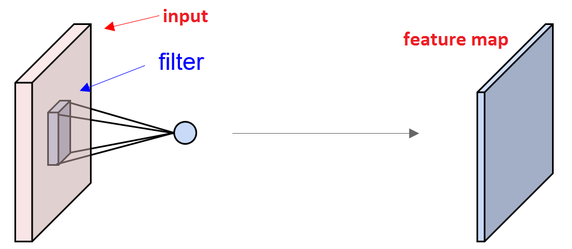
\includegraphics[width=8cm]{cnn_architecture.png}
\centering
\caption{Picture created by Anirban Ray, Quora}
\end{figure}

\end{document}